\section{Evaluarea rezultatelor}

Evaluarea predictorului OGEHL a fost realizata pe benchmark-ul \textbf{applu}
din suita Stanford, simuland \textbf{500 de milioane de instructiuni} cu
simulatorul \textit{sim-bpred} din SimpleScalar. Au fost testate 9 configuratii
(c1--c9) care variaza sistematic cei trei parametri configurabili: numarul de
tabele ($N$), marimea tabelelor ($S$) si lungimea contoarelor ($k$). Metrica
principala utilizata este \textbf{rata de predictie corecta a directiei}
(\textit{bpred\_dir\_rate}).

\subsection{Configuratiile testate}

\begin{table}[H]
    \centering
    \small
    \begin{tabular}{|c|c|c|c|c|}
        \hline
        \textbf{Config} & \textbf{Tabele ($N$)} & \textbf{Marime tabel ($S$)} & \textbf{Biti contor ($k$)} & \textbf{Acuratete} \\
        \hline
        c1 & 4  & 512   & 3 & 75.24\% \\
        c2 & 4  & 2048  & 4 & 97.54\% \\
        c3 & 7  & 512   & 3 & 68.42\% \\
        c4 & 7  & 2048  & 4 & 97.36\% \\
        c5 & 7  & 2048  & 5 & 98.37\% \\
        c6 & 7  & 8192  & 4 & 98.37\% \\
        c7 & 12 & 2048  & 4 & 95.58\% \\
        c8 & 12 & 8192  & 4 & 97.55\% \\
        c9 & 12 & 8192  & 5 & 98.37\% \\
        \hline
    \end{tabular}
    \caption{Rezultatele celor 9 configuratii OGEHL pe benchmark-ul applu}
    \label{tab:eval_results}
\end{table}

\begin{figure}[H]
    \centering
    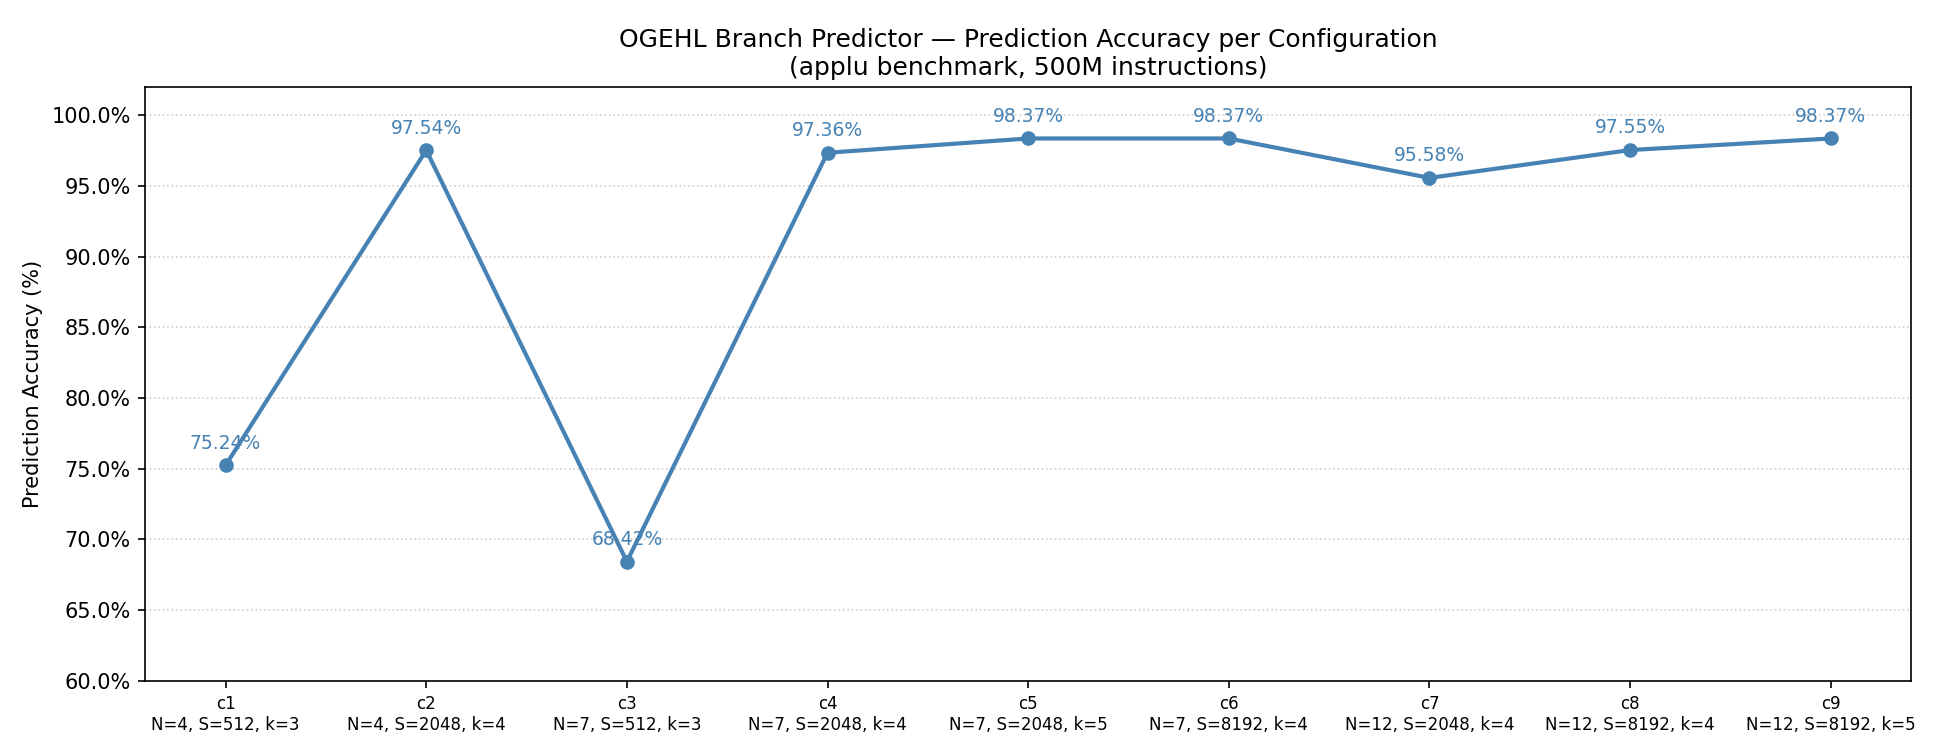
\includegraphics[width=\linewidth]{images/applu_graph.png}
    \caption{Acuratetea predictorului OGEHL per configuratie (benchmark applu)}
    \label{fig:eval_graph}
\end{figure}

\subsection{Analiza rezultatelor}

\subsubsection*{Impactul marimii tabelelor}

Cel mai puternic factor care influenteaza acuratetea este \textbf{marimea
tabelelor}. Configuratiile cu $S = 512$ (c1 si c3) produc rezultatele cele mai
slabe: 75.24\%, respectiv 68.42\%. La aceasta dimensiune, tabelele sunt
suprasolicitate --- mai multe branch-uri diferite indexeaza acelasi contor
(\textit{aliasing}), degradand semnificativ calitatea predictiei.

Trecerea de la $S = 512$ la $S = 2048$ produce un salt dramatic de acuratete
(de exemplu, de la 75.24\% la 97.54\% intre c1 si c2), confirmand ca
\textbf{aliasing-ul este principala sursa de erori} la configuratii mici.
Cresterea ulterioara la $S = 8192$ aduce inca un castig modest, dar consistent,
de aproximativ 1 punct procentual.

\subsubsection*{Impactul lungimii contoarelor}

Cresterea lungimii contoarelor de la $k = 4$ la $k = 5$ biti aduce un castig
uniform de \textbf{$\approx$1\%} acuratete in toate configuratiile comparabile:

\begin{itemize}
    \item c4 ($k=4$): 97.36\% $\rightarrow$ c5 ($k=5$): 98.37\% \quad ($+1.01$pp)
    \item c8 ($k=4$): 97.55\% $\rightarrow$ c9 ($k=5$): 98.37\% \quad ($+0.82$pp)
\end{itemize}

Contoarele mai lungi sunt mai rezistente la schimbari de comportament tranzitorii,
reducand rata de mispredictii in special pentru branch-urile cu comportament
predominant unidirectional.

\subsubsection*{Impactul numarului de tabele}

Rezultatele arata ca \textbf{mai multe tabele nu implica neaparat acuratete mai
mare} daca marimea tabelelor nu este si ea adaptata. Configuratia c7
($N=12$, $S=2048$, $k=4$) obtine doar 95.58\%, mai slab decat c4 ($N=7$,
$S=2048$, $k=4$) cu 97.36\%. Aceasta se explica prin faptul ca un numar mai
mare de tabele cu aceeasi dimensiune totala de memorie inseamna tabele mai
mici effective per nivel de istorie, crescand aliasing-ul.

Cresterea $S$ la 8192 (c8) recupereaza partial aceasta pierdere (97.55\%),
iar adaugarea $k=5$ (c9) atinge optimul de 98.37\%.

\subsubsection*{Configuratia optima}

Trei configuratii ating aceeasi acuratete maxima de \textbf{98.37\%}:
c5 ($N=7$, $S=2048$, $k=5$), c6 ($N=7$, $S=8192$, $k=4$) si
c9 ($N=12$, $S=8192$, $k=5$). Dintre acestea, \textbf{c5} este cea mai
eficienta din punct de vedere al memoriei: 7 tabele $\times$ 2048 intrari
$\times$ 5 biti = $\approx$90~KB, comparativ cu c6 sau c9 care necesita
de 4 ori mai multa memorie pentru acelasi rezultat.

\subsection{Concluzii privind parametrii}

\begin{enumerate}
    \item \textbf{Marimea tabelelor} este parametrul cu cel mai mare impact.
          Sub 2048 intrari, aliasing-ul domina si acuratetea scade dramatic.
    \item \textbf{Lungimea contoarelor} de 5 biti ofera un castig consistent
          de $\approx$1\% fata de 4 biti, la un cost de memorie marginal.
    \item \textbf{Numarul de tabele} trebuie corelat cu marimea tabelelor;
          7 tabele reprezinta echilibrul optim pentru marimile de tabel testate.
\end{enumerate}

% ================================================================
\subsection{Benchmark mgrid}

Cel de-al doilea benchmark folosit este \textbf{mgrid}, o aplicatie de rezolvare
a ecuatiilor pe grile multi-nivel (multigrid solver), cu un profil de executie
predominant numeric si bucle regulate. Spre deosebire de applu, mgrid prezinta
un comportament de ramificatii mult mai predictibil, ceea ce se reflecta direct
in rezultate.

\begin{table}[H]
    \centering
    \small
    \begin{tabular}{|c|c|c|c|c|}
        \hline
        \textbf{Config} & \textbf{Tabele ($N$)} & \textbf{Marime tabel ($S$)} & \textbf{Biti contor ($k$)} & \textbf{Acuratete} \\
        \hline
        c1 & 4  & 512   & 3 & 99.20\% \\
        c2 & 4  & 2048  & 4 & 99.21\% \\
        c3 & 7  & 512   & 3 & 99.19\% \\
        c4 & 7  & 2048  & 4 & 99.21\% \\
        c5 & 7  & 2048  & 5 & 99.21\% \\
        c6 & 7  & 8192  & 4 & 99.21\% \\
        c7 & 12 & 2048  & 4 & 99.20\% \\
        c8 & 12 & 8192  & 4 & 99.21\% \\
        c9 & 12 & 8192  & 5 & 99.21\% \\
        \hline
    \end{tabular}
    \caption{Rezultatele celor 9 configuratii OGEHL pe benchmark-ul mgrid}
    \label{tab:mgrid_results}
\end{table}

\begin{figure}[H]
    \centering
    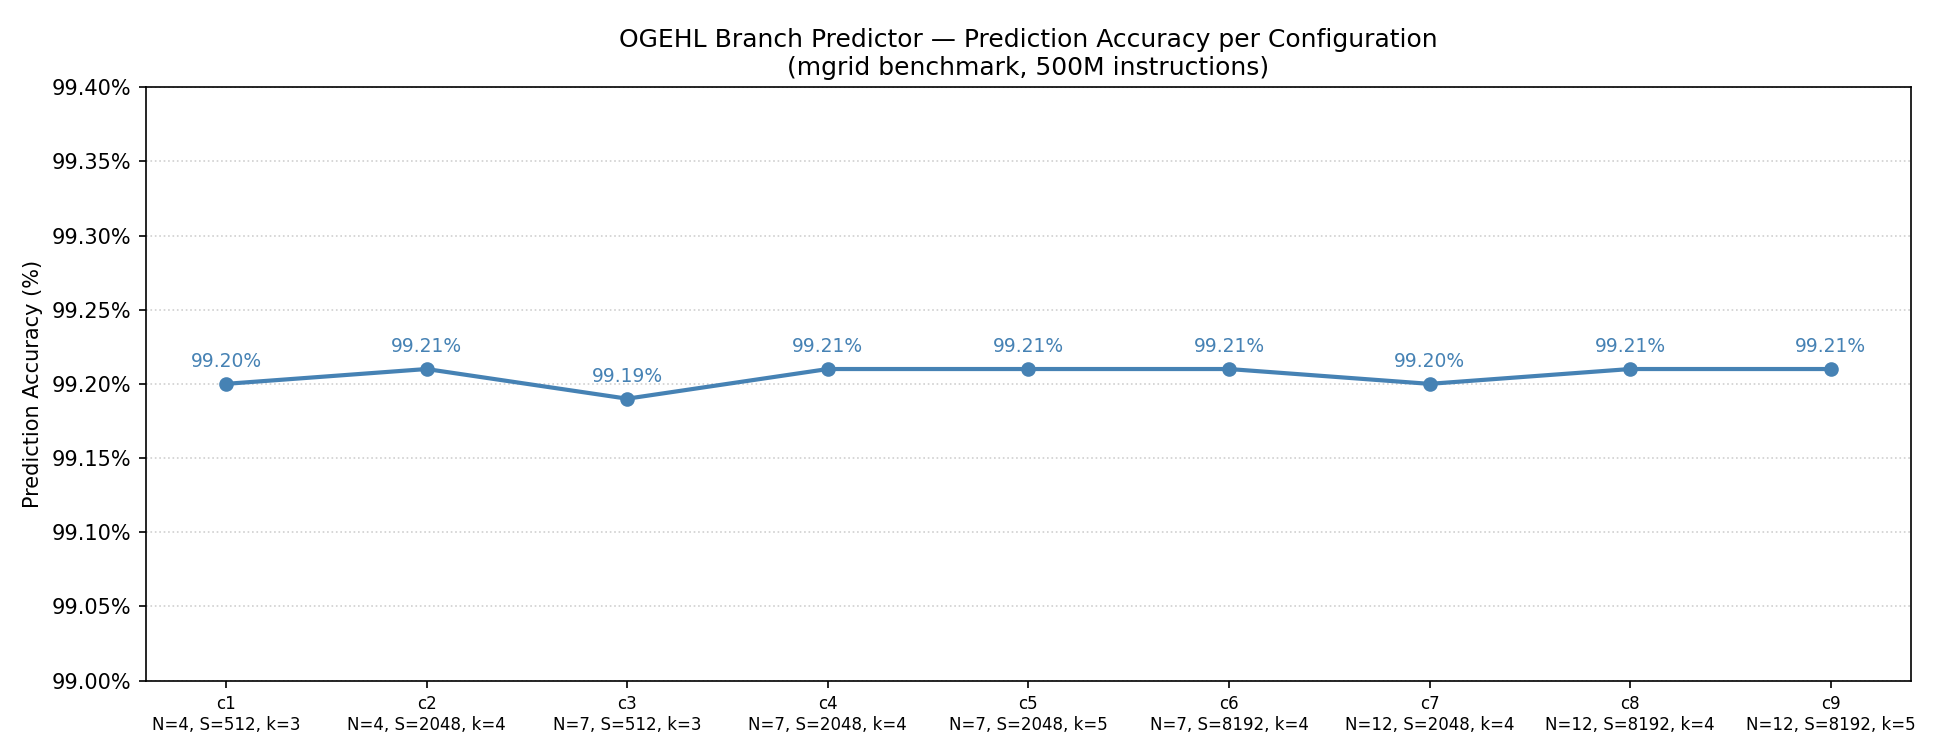
\includegraphics[width=\linewidth]{images/mgrid_graph.png}
    \caption{Acuratetea predictorului OGEHL per configuratie (benchmark mgrid)}
    \label{fig:mgrid_graph}
\end{figure}

\subsubsection*{Analiza rezultatelor mgrid}

Primul lucru care iese in evidenta este intervalul extrem de ingust de variatie
a acuratetii: \textbf{99.19\%--99.21\%}, o diferenta maxima de doar 0.02 puncte
procentuale intre cea mai slaba si cea mai buna configuratie. Aceasta uniformitate
este o caracteristica a benchmark-ului in sine: mgrid are un numar relativ mic de
branch-uri per instructiune si aproape toate sunt puternic bias towards
\textit{taken}, ceea ce face ca orice configuratie rezonabila a predictorului sa
le ghiceasca corect.

Spre deosebire de applu, unde configuratiile cu $S=512$ colapsau la 68--75\%
din cauza aliasing-ului masiv, pe mgrid \textbf{chiar si c1 si c3 ating 99.19\%}.
Numarul mic de branch-uri unice (2.24 milioane fata de 14.6 milioane in applu)
inseamna ca tabelele de 512 intrari sunt suficiente pentru a acoperi majoritatea
branch-urilor fara coliziuni semnificative.

Parametrii $N$, $S$ si $k$ au un efect practic neglijabil pe acest tip de aplicatie:
predictorul OGEHL este deja saturat la acuratete maxima inca de la configuratia
minima. Acesta este un comportament asteptat pentru programe cu structuri de
control regulate si predictibile (bucle cu numar fix de iteratii, fara conditii
complexe dependente de date).

\subsubsection*{Comparatie applu vs mgrid}

\begin{table}[H]
    \centering
    \small
    \begin{tabular}{|l|c|c|c|}
        \hline
        \textbf{Benchmark} & \textbf{Acuratete min} & \textbf{Acuratete max} & \textbf{Variatie} \\
        \hline
        applu & 68.42\% (c3) & 98.37\% (c5/c6/c9) & 29.95 pp \\
        mgrid & 99.19\% (c3) & 99.21\% (c2/c4--c9) & 0.02 pp \\
        \hline
    \end{tabular}
    \caption{Comparatie acuratete OGEHL: applu vs mgrid}
    \label{tab:compare}
\end{table}

Cele doua benchmark-uri ilustreaza doua extreme ale spectrului de dificultate
pentru un predictor de ramificatii. \textbf{applu} este sensibil la configuratie
si expune clar limitele arhitecturii la dimensiuni mici de tabel, oferind un
cadru de evaluare relevant pentru optimizarea parametrilor. \textbf{mgrid} este
practic insensibil la parametri, confirma ca implementarea functioneaza corect,
dar nu ofera putere discriminatorie intre configuratii.

% ================================================================
\subsection{Benchmark compress}

\textbf{compress} este un benchmark de compresie/decompresie (LZW), cu un profil
de executie dominat de bucle de procesare a datelor si ramificatii dependente de
continutul fisierului de intrare. Spre deosebire de mgrid, comportamentul
branch-urilor depinde puternic de datele procesate, ceea ce face predicatia mai
dificila si evidentiaza diferente intre configuratii.

\begin{table}[H]
    \centering
    \small
    \begin{tabular}{|c|c|c|c|c|}
        \hline
        \textbf{Config} & \textbf{Tabele ($N$)} & \textbf{Marime tabel ($S$)} & \textbf{Biti contor ($k$)} & \textbf{Acuratete} \\
        \hline
        c1 & 4  & 512   & 3 & 87.72\% \\
        c2 & 4  & 2048  & 4 & 84.00\% \\
        c3 & 7  & 512   & 3 & 83.46\% \\
        c4 & 7  & 2048  & 4 & 83.46\% \\
        c5 & 7  & 2048  & 5 & 89.37\% \\
        c6 & 7  & 8192  & 4 & 83.46\% \\
        c7 & 12 & 2048  & 4 & 83.46\% \\
        c8 & 12 & 8192  & 4 & 83.46\% \\
        c9 & 12 & 8192  & 5 & 89.90\% \\
        \hline
    \end{tabular}
    \caption{Rezultatele celor 9 configuratii OGEHL pe benchmark-ul compress}
    \label{tab:compress_results}
\end{table}

\begin{figure}[H]
    \centering
    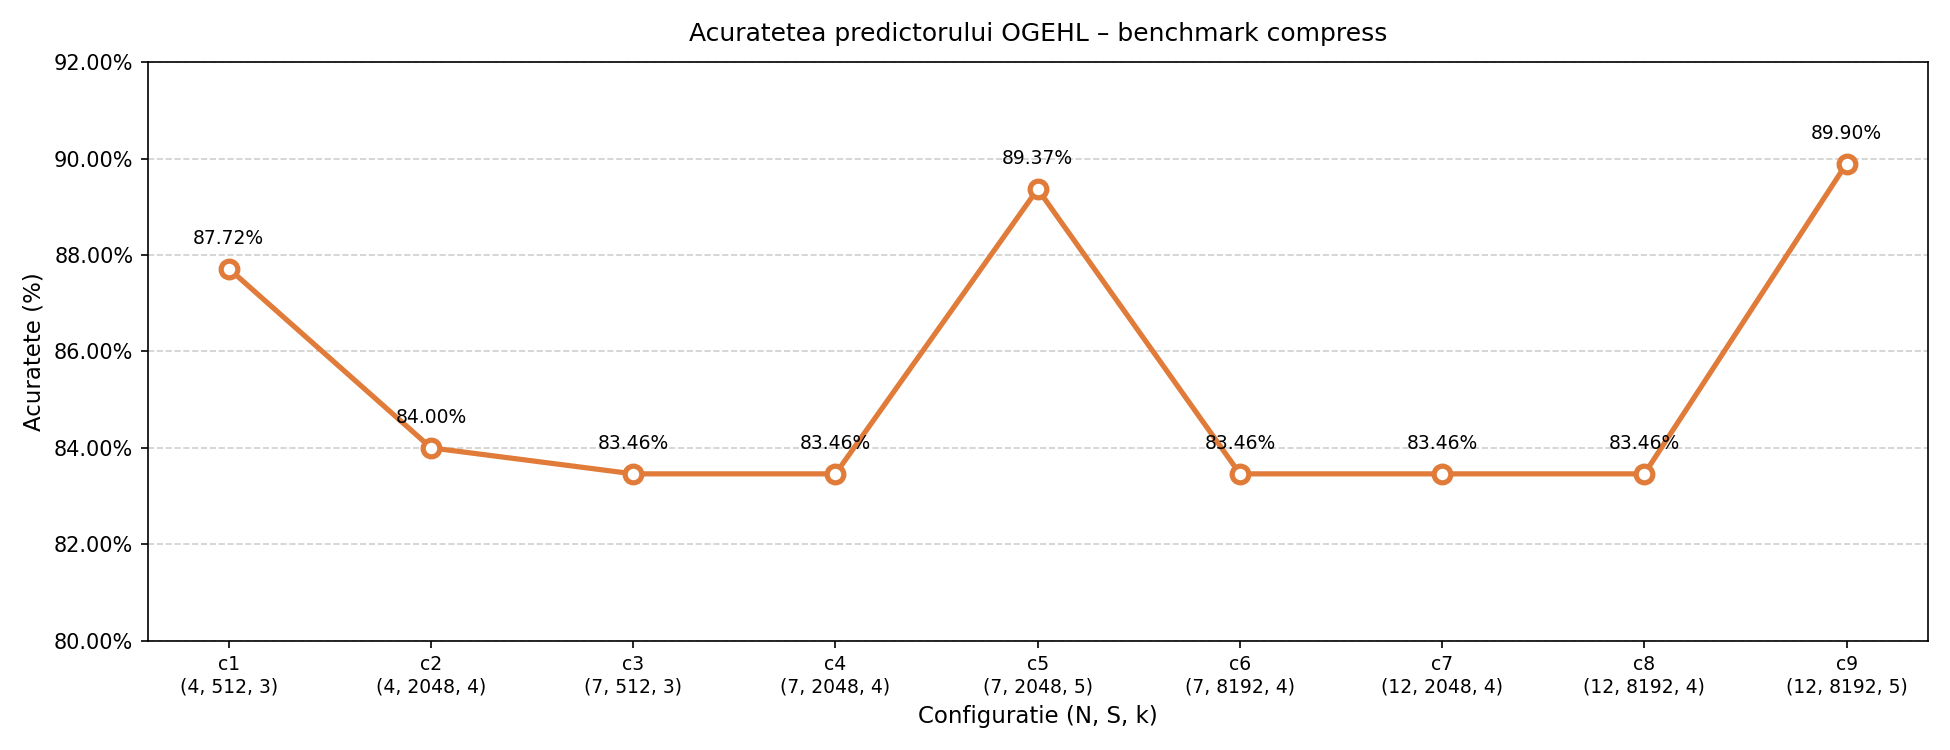
\includegraphics[width=\linewidth]{images/compress_graph.png}
    \caption{Acuratetea predictorului OGEHL per configuratie (benchmark compress)}
    \label{fig:compress_graph}
\end{figure}

\subsubsection*{Analiza rezultatelor compress}

Primul aspect remarcabil este comportamentul \textbf{aparent contraintuitiv} al
configuratiei c1 ($N=4$, $S=512$, $k=3$), care obtine \textbf{87.72\%} ---
mai mult decat c2 ($N=4$, $S=2048$, $k=4$, 84.00\%) sau c4 (83.46\%). Aceasta
anomalie sugereaza ca pe compress, cresterea numarului de tabele si a dimensiunii
lor \textit{fara cresterea lungimii contoarelor} poate introduce instabilitate:
mai multe contexte de istorie diferite ajung sa indexeze aceleasi ramificatii,
iar contoarele de 4 biti nu sunt suficient de rezistente pentru a gestiona
corect conflictele.

\textbf{Lungimea contoarelor} ($k$) este factorul decisiv pe acest benchmark.
Toate configuratiile cu $k=4$ converg la aceeasi acuratete de 83.46\%, indiferent
de $N$ si $S$. Cresterea la $k=5$ produce un salt semnificativ:

\begin{itemize}
    \item c5 ($N=7$, $S=2048$, $k=5$): 89.37\% \quad ($+5.91$pp fata de c4)
    \item c9 ($N=12$, $S=8192$, $k=5$): 89.90\% \quad ($+6.44$pp fata de c8)
\end{itemize}

Aceasta indica faptul ca pe compress, branch-urile au un comportament oscilant
mai pronuntat, iar contoarele scurte ($k=4$) se satureaza sau se desatureaza
prea rapid, producand mispredictii repetate. Contoarele de 5 biti ofera o
inertie mai mare, reducand rata de eroare.

Configuratia optima pentru compress este \textbf{c9} ($N=12$, $S=8192$, $k=5$)
cu 89.90\%, urmata indeaproape de c5 (89.37\%), care este insa mult mai eficienta
din punct de vedere al memoriei.

% ================================================================
\subsection{Benchmark ijpeg}

\textbf{ijpeg} este un benchmark de compresie JPEG, cu un profil de executie
intensiv computatonal (transformate DCT, cuantizare, codare Huffman). Ramificatiile
sale sunt partial predictibile --- structuri de control ale buclelor de procesare
a blocurilor de pixeli --- dar includ si conditii dependente de date (valorile
coeficientilor DCT), ceea ce produce o acuratete intermediara.

\begin{table}[H]
    \centering
    \small
    \begin{tabular}{|c|c|c|c|c|}
        \hline
        \textbf{Config} & \textbf{Tabele ($N$)} & \textbf{Marime tabel ($S$)} & \textbf{Biti contor ($k$)} & \textbf{Acuratete} \\
        \hline
        c1 & 4  & 512   & 3 & 93.53\% \\
        c2 & 4  & 2048  & 4 & 93.76\% \\
        c3 & 7  & 512   & 3 & 93.26\% \\
        c4 & 7  & 2048  & 4 & 93.65\% \\
        c5 & 7  & 2048  & 5 & 93.65\% \\
        c6 & 7  & 8192  & 4 & 94.00\% \\
        c7 & 12 & 2048  & 4 & 93.47\% \\
        c8 & 12 & 8192  & 4 & 94.00\% \\
        c9 & 12 & 8192  & 5 & 94.00\% \\
        \hline
    \end{tabular}
    \caption{Rezultatele celor 9 configuratii OGEHL pe benchmark-ul ijpeg}
    \label{tab:ijpeg_results}
\end{table}

\begin{figure}[H]
    \centering
    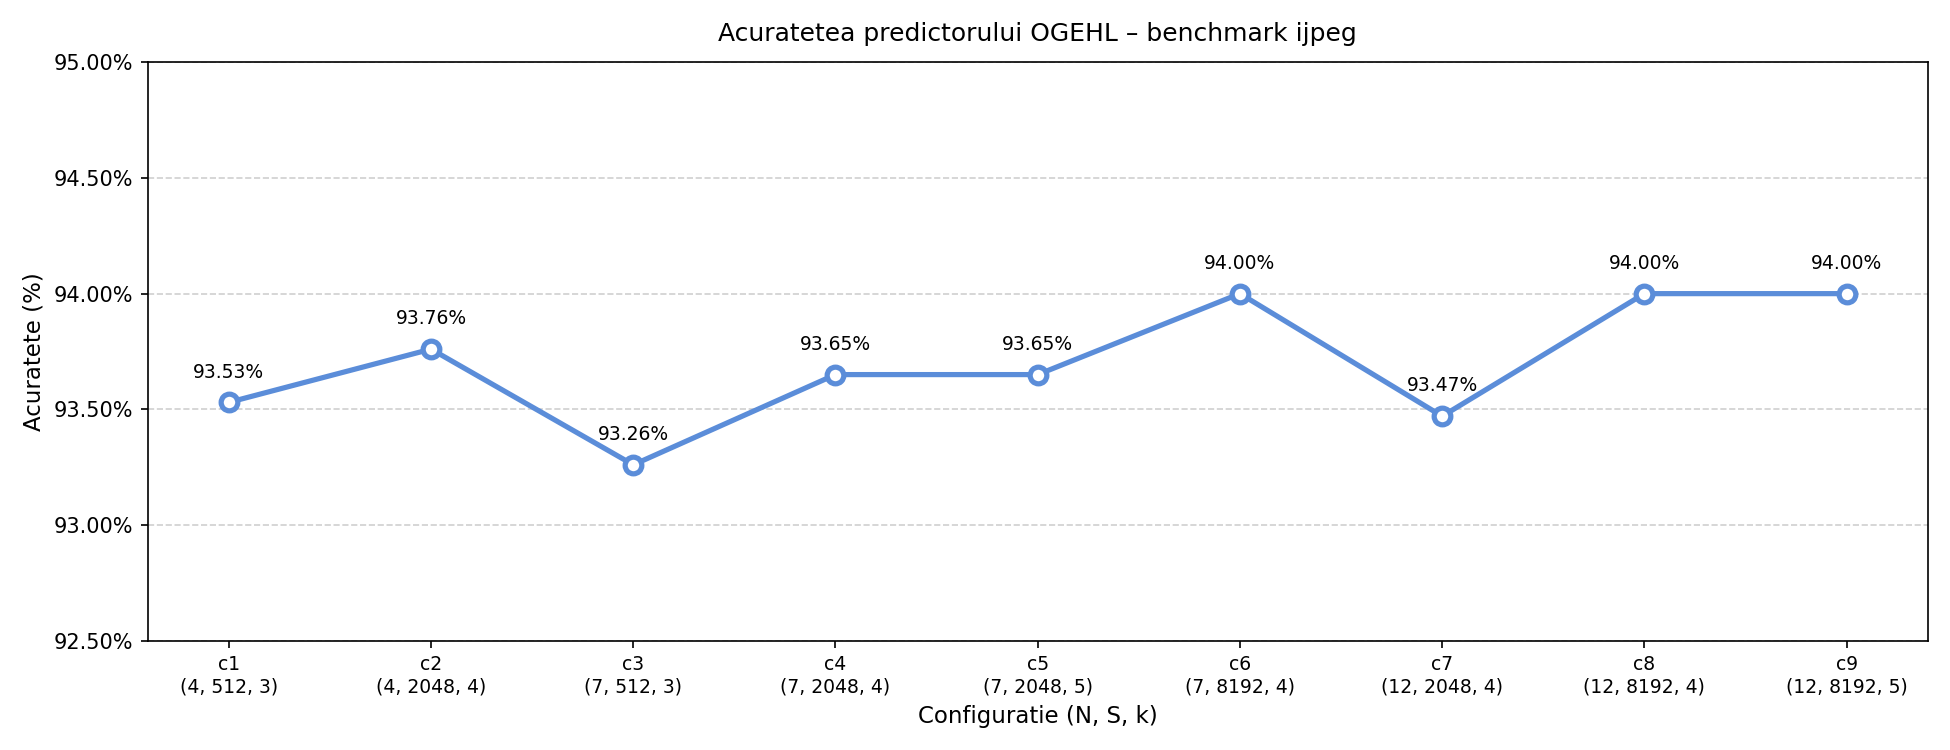
\includegraphics[width=\linewidth]{images/ijpeg_graph.png}
    \caption{Acuratetea predictorului OGEHL per configuratie (benchmark ijpeg)}
    \label{fig:ijpeg_graph}
\end{figure}

\subsubsection*{Analiza rezultatelor ijpeg}

Intervalul de variatie al acuratetii este \textbf{93.26\%--94.00\%} (0.74~pp),
mai ingust decat applu (29.95~pp) dar mai larg decat mgrid (0.02~pp). Aceasta
plaseaza ijpeg intr-o categorie intermediara: benchmark-ul are suficiente
ramificatii predictibile pentru a oferi o acuratete ridicata chiar si la
configuratii mici, dar destule ramificatii dependente de date pentru a
discrimina intre configuratii.

\textbf{Marimea tabelelor} are un impact moderat si consistent: configuratia
c6 si c8 ($S=8192$) ating ambele 94.00\%, fata de 93.65\% pentru c4 ($S=2048$).
In schimb, \textbf{lungimea contoarelor} are un efect neglijabil: c5 ($k=5$)
obtine acelasi scor ca c4 ($k=4$, 93.65\%), iar c9 ($k=5$) la fel ca c8
($k=4$, 94.00\%). Pe ijpeg, erorile de predictie sunt cauzate mai ales de
aliasing si nu de instabilitatea contoarelor.

Configuratia minima cu cel mai bun raport memorie/acuratete este \textbf{c6}
($N=7$, $S=8192$, $k=4$) cu 94.00\%, aceeasi acuratete ca c8 si c9 care
folosesc de 1.7$\times$ mai multa memorie (12 tabele vs.\ 7).

% ================================================================
\subsection{Comparatie globala a celor patru benchmark-uri}

\begin{table}[H]
    \centering
    \small
    \begin{tabular}{|l|c|c|c|c|}
        \hline
        \textbf{Benchmark} & \textbf{Acuratete min} & \textbf{Acuratete max} & \textbf{Variatie} & \textbf{Config optima} \\
        \hline
        applu    & 68.42\% (c3) & 98.37\% (c5/c6/c9) & 29.95 pp & c5 \\
        mgrid    & 99.19\% (c3) & 99.21\% (c2/c4--c9)&  0.02 pp & orice \\
        compress & 83.46\% (c3--c8) & 89.90\% (c9)   &  6.44 pp & c9 / c5 \\
        ijpeg    & 93.26\% (c3) & 94.00\% (c6/c8/c9) &  0.74 pp & c6 \\
        \hline
    \end{tabular}
    \caption{Comparatie acuratete OGEHL pe toate cele patru benchmark-uri}
    \label{tab:compare_all}
\end{table}

Rezultatele globale confirma ca predictorul OGEHL se comporta diferit in functie
de natura benchmark-ului. Pe \textbf{mgrid}, acuratetea ridicata si invarianta
confirma corectitudinea implementarii. Pe \textbf{applu}, sensibilitatea ridicata
la parametri ofera cel mai relevant cadru de evaluare. Pe \textbf{compress},
lungimea contoarelor devine factorul critic, reflectand comportamentul oscilant al
ramificatiilor dependente de date. Pe \textbf{ijpeg}, marimea tabelelor conteaza
mai mult decat numarul lor, iar valoarea $k$ are impact minim.
